\subsection{Common-Emitter Amplifier with Fixed Bias Circuit}

\begin{figure}[H]
    \centering
    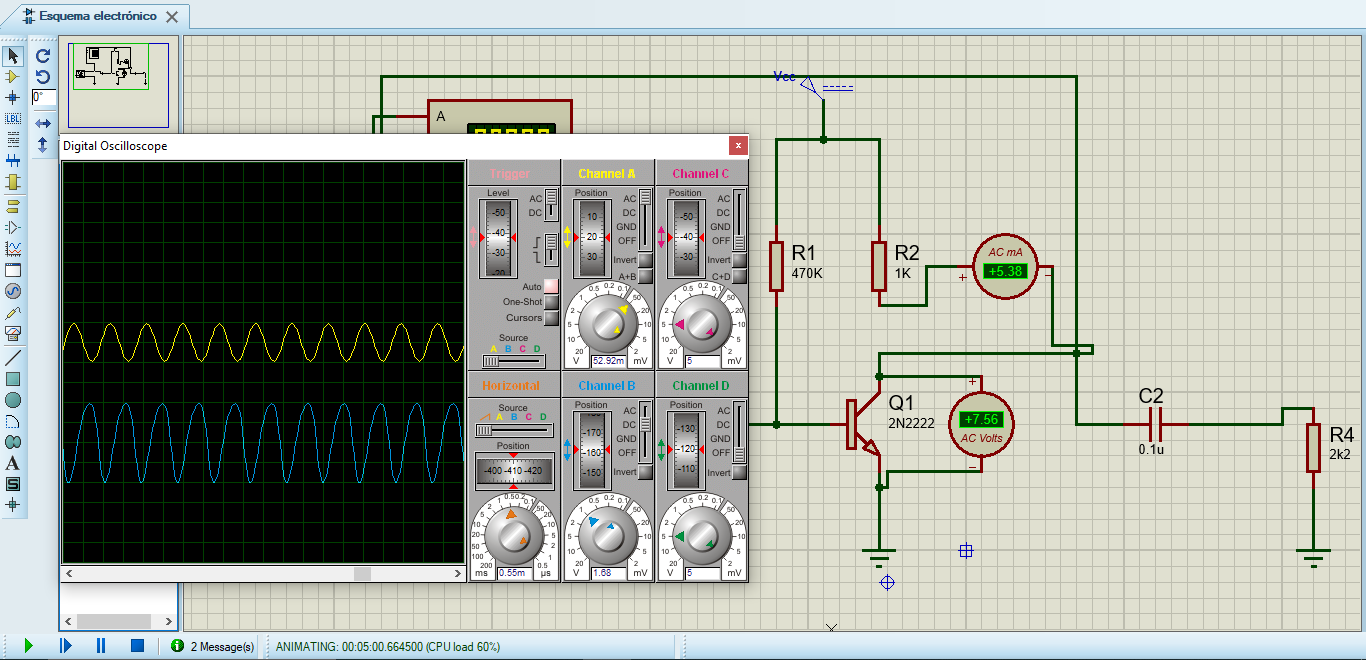
\includegraphics[width = 0.9\textwidth]{Imagenes/Imagenes_Juan/Circuito1_Simulado.PNG}
    \caption{Common-Emitter Amplifier with Fixed Bias Circuit}
    \label{circuit1Simulated}
\end{figure}

Measurements:
\begin{center}
    Q(7.56 V, 5.37 mA).
    
\end{center}
Oscilloscope:

\begin{center}
    Input = 100mVpp, Output = 5.28Vpp
\end{center}

\newpage

\subsection{Common-Emitter Amplifier with Emitter-Stabilized Bias Circuit}

\begin{figure}[H]
    \centering
    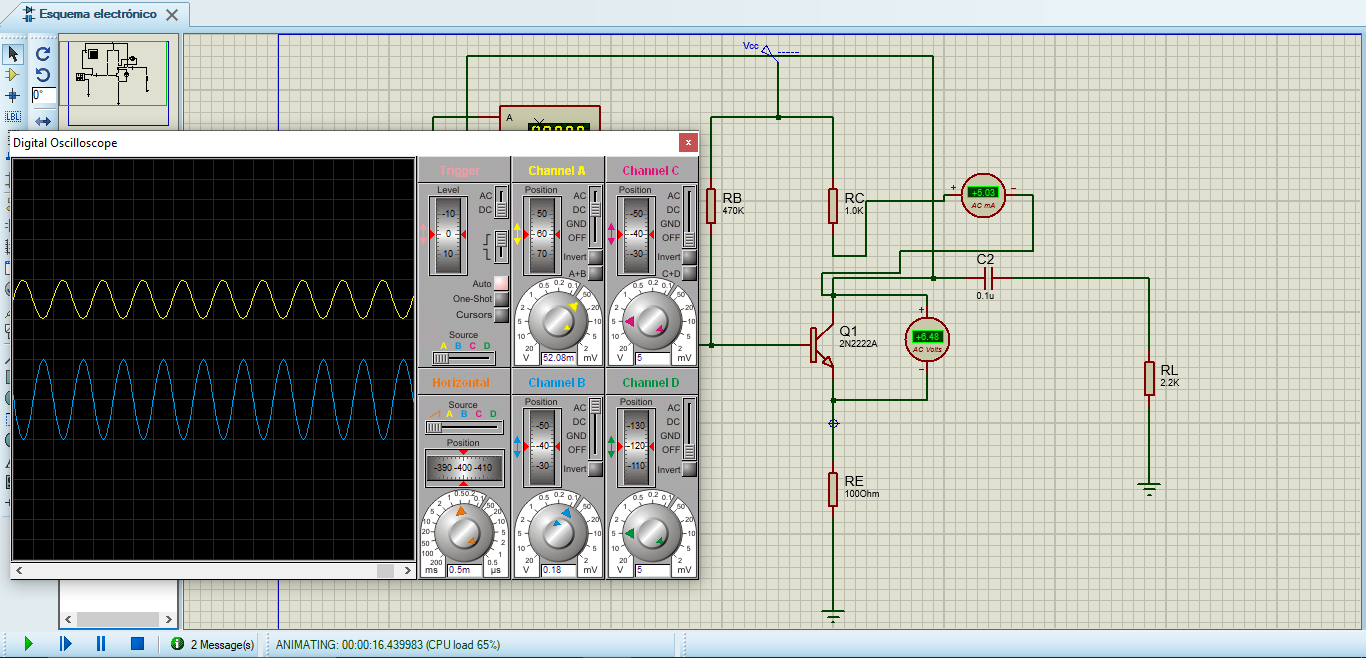
\includegraphics[width = 0.9\textwidth]{Imagenes/Imagenes_Juan/Circuito2_Simulado.PNG}
    \caption{Common-Emitter Amplifier with Emitter-Stabilized Bias Circuit}
    \label{circuit2Simulated}
\end{figure}

Measurements:
\begin{center}
    Q( 7.56V, 5.35 mA)
\end{center}

Oscilloscope:

\begin{center}
    Input = 104 mV, Output = 720 mV
\end{center}